\begin{frame}
  \frametitle{Summary}
  \textbf{Pre-detonation nuclear forensics analysis on SNF}
  \begin{minipage}{0.35\textwidth}
    \begin{figure}
      \centering
      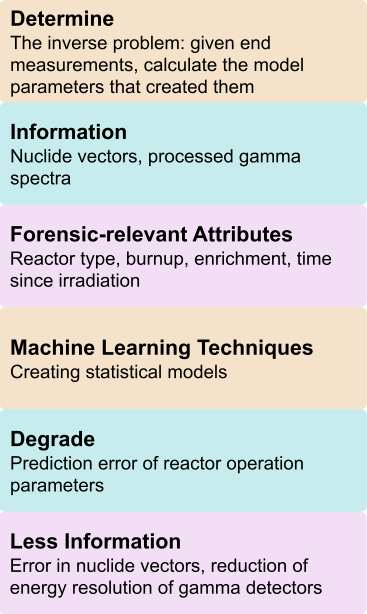
\includegraphics[height=0.7\textheight]{./figures/overview.png}
    \end{figure}
  \end{minipage}%
  \begin{minipage}{0.65\textwidth}
  \begin{itemize}
    \item Demonstrated:
    \begin{itemize}
      \item Simulation of training data set
      \item Information reduction of training set
      \item Prediction of reactor type, burnup, enrichment, and time since irradiation via:
        \begin{itemize}
          \item Maximum Log-Likelihood Calculations
          \item \textit{k}-Nearest Neighbors
          \item Decision Trees
        \end{itemize}
      \item Initial analysis of predictions with respect to information reduction
    \end{itemize}
    \item Simplifications:
    \begin{itemize}
    % TODO fix me
      \item No deep inquiry regarding feature reduction
      \item No physically based information reduction
      \item Missing summary metrics for likelihood method
    \end{itemize}
  \end{itemize}
  \end{minipage}
\end{frame}

%\begin{frame}
%  \frametitle{ddd}
%  \textbf{dd}\\
%  dd \\~\\
%\end{frame}

% feature reduction, and or only using matching nuclides?
% sfcompo, get to work with new alg?
% baselines for plots
% metrics, esp accuracy
% rerun algs with 100% db tested, or do same small test set across all methods?
% Energy window discussion: How many to include, How wide for each detector, Manual, semi-manual, automatic

